\documentclass[]{article}
\usepackage{lmodern}
\usepackage{amssymb,amsmath}
\usepackage{ifxetex,ifluatex}
\usepackage{fixltx2e} % provides \textsubscript
\ifnum 0\ifxetex 1\fi\ifluatex 1\fi=0 % if pdftex
  \usepackage[T1]{fontenc}
  \usepackage[utf8]{inputenc}
\else % if luatex or xelatex
  \ifxetex
    \usepackage{mathspec}
  \else
    \usepackage{fontspec}
  \fi
  \defaultfontfeatures{Ligatures=TeX,Scale=MatchLowercase}
\fi
% use upquote if available, for straight quotes in verbatim environments
\IfFileExists{upquote.sty}{\usepackage{upquote}}{}
% use microtype if available
\IfFileExists{microtype.sty}{%
\usepackage[]{microtype}
\UseMicrotypeSet[protrusion]{basicmath} % disable protrusion for tt fonts
}{}
\PassOptionsToPackage{hyphens}{url} % url is loaded by hyperref
\usepackage[unicode=true]{hyperref}
\hypersetup{
            pdfborder={0 0 0},
            breaklinks=true}
\urlstyle{same}  % don't use monospace font for urls
\usepackage{graphicx,grffile}
\makeatletter
\def\maxwidth{\ifdim\Gin@nat@width>\linewidth\linewidth\else\Gin@nat@width\fi}
\def\maxheight{\ifdim\Gin@nat@height>\textheight\textheight\else\Gin@nat@height\fi}
\makeatother
% Scale images if necessary, so that they will not overflow the page
% margins by default, and it is still possible to overwrite the defaults
% using explicit options in \includegraphics[width, height, ...]{}
\setkeys{Gin}{width=\maxwidth,height=\maxheight,keepaspectratio}
\IfFileExists{parskip.sty}{%
\usepackage{parskip}
}{% else
\setlength{\parindent}{0pt}
\setlength{\parskip}{6pt plus 2pt minus 1pt}
}
\setlength{\emergencystretch}{3em}  % prevent overfull lines
\providecommand{\tightlist}{%
  \setlength{\itemsep}{0pt}\setlength{\parskip}{0pt}}
\setcounter{secnumdepth}{0}
% Redefines (sub)paragraphs to behave more like sections
\ifx\paragraph\undefined\else
\let\oldparagraph\paragraph
\renewcommand{\paragraph}[1]{\oldparagraph{#1}\mbox{}}
\fi
\ifx\subparagraph\undefined\else
\let\oldsubparagraph\subparagraph
\renewcommand{\subparagraph}[1]{\oldsubparagraph{#1}\mbox{}}
\fi

% set default figure placement to htbp
\makeatletter
\def\fps@figure{htbp}
\makeatother


\date{}

\begin{document}

\section{Rapport Projet Deuxième
Année}\label{rapport-projet-deuxiuxe8me-annuxe9e}

\subsection{1) Le reseau TOR}\label{le-reseau-tor}

\subsubsection{a) Qu'est ce que c'est ?}\label{a-quest-ce-que-cest}

\begin{verbatim}
TOR est l'accronyme de The Onion Router.  Le réseau a été concu par la marine américaine dans le but de protéger les communications gouvernamentales pendant les opérations secrètes. Le département de la défence a financé le projet a plus de 60% tandis que les autres financements proviennent des organisations qui protègent la vie privée tel que des associations de journalistes, des groupes d'activistes ou l'EFF.  TOR est désormais une organisation a but non lucratif qui se concentre sur la protection des données personnelles et l'anonymat des internautes sur le web. C'est un projet open source, c'est a dire que tout le monde peut voir le code et le corriger si nécessaire.
\end{verbatim}

\begin{figure}
\centering
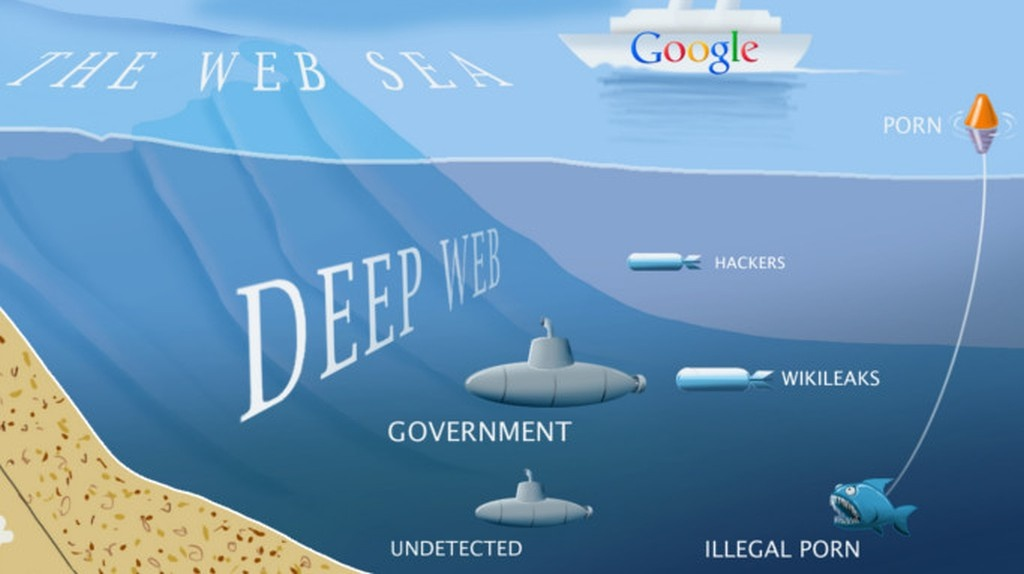
\includegraphics{./tex2pdf.4104/6d479c0a3a7130cebbf480e114702b120ce3f3bb.jpg}
\caption{L'internet profond}
\end{figure}

\begin{verbatim}
Le reseau TOR permet d'accéder au *"DEEP WEB"* ou l'internet profond. Comme cela est illustré dans la figure précédente, une partie du réseau internet est enfouie, inaccesible depuis les moteurs de recherche communs tels que GOOGLE, SAFARI... Le deep web correspond a tout ce qui n'est pas indexé par ces moteurs de recherche.  C'est biensur le repère de tout commerce illégal. Par exemple, en octobre 2013, Silk Road, site de traffic de drogue trouvable uniquement sur le deep web a été "trouvé" et fermé. C'est aussi le repère des organisations gouvernamentales ou des groupes d'activistes.
\end{verbatim}

\subsubsection{b) Comment TOR garde
l'anonymat?}\label{b-comment-tor-garde-lanonymat}

\begin{verbatim}
L'objectif de TOR est que l'utilisateur puisse utiliser internet tout en restant totalement anonyme. Pour cela, il faut que personne ne soit capable de retrouver la source de la demande ou la destination de l'information.
Lorsque nous nous connectons à un site web, notre ordinateur essaie de se connecter directement à son serveur par la route la plus courte. Ce qui prime est la rapidité et l'efficacité. Notre adresse IP est donc recensée comme point de départ de la communication et il n'y a aucun anonymat.
\end{verbatim}

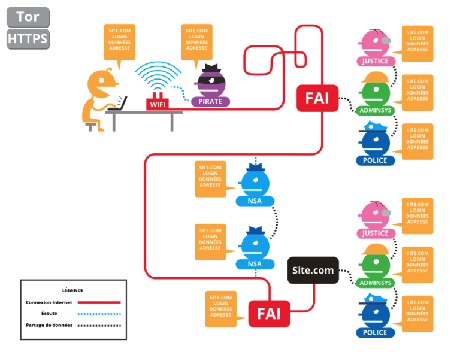
\includegraphics{images/Connexion_classique.png} Toute personne ayant
accès à la requête connait l'emetteur, le destinataire et les données.

\begin{verbatim}
 Pour éviter cela, TOR rompt celle ligne entre notre ordinateur et ce serveur distant. TOR utilise l'Onion Routing qui est une technique de communication anonyme sur un réseau. Les messages sont chiffrés en continu en passant de noeuds en noeuds. Ces noeuds sont aussi appelés routeurs Onions. Le terme onion se réfère aux différentes couches de chiffrement effectuées par des relais anonymes qui protègent les messages. Le routage devient alors totalement invisible.

Si une personne A envoie une requête au serveur B, la requête va passer par plusieurs noeuds. Cette requête va d'abbord être chiffrer avec le clé publique du noeuds de sortie puis re-chiffrer par la clé publique de l'avant dernier noeud et ainsi de suite jusqu'au premier noeud auquel elle va être envoyé. Ce principe permet que le premier noeud connaisse seulement l'expéditeur mais pas la destination, les noeuds intermédiaires ne connaissent que le noeuds précédent et le suivant et le noeud de sortie ne connait que le destinataire.
Tor utilise ce même chemin pendant plusieurs minutes puis le change pour qu'aucun lien ne puisse être établi.
\end{verbatim}

\begin{figure}
\centering
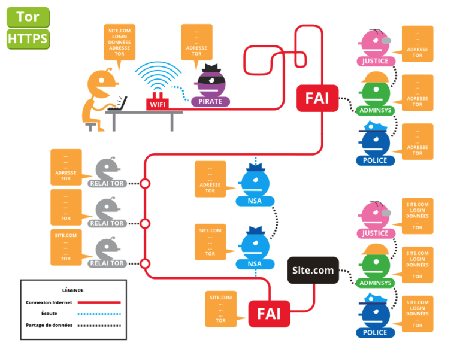
\includegraphics{images/connexion_tor.png}
\caption{Connexion à internet classique avec TOR et HTTPS}
\end{figure}

\subsection{2) Familiarisation avec les
technologies}\label{familiarisation-avec-les-technologies}

\subsubsection{a)Markdown}\label{amarkdown}

\begin{verbatim}
  un language simple et léger basé sur un balisage moins lourd que celui utilisé pour html. Utilisé à la base pour écrire un document html il a été adapté et permet aujourd'hui via l'intermédiaire de Pandoc (décrit ci-dessous) de créer
  à partir d'un document .md une multitude de document tel que .doc , .odt...
  Ce language permet une grande facilité de lecture et d'écriture.
\end{verbatim}

\subsubsection{b)Pandoc}\label{bpandoc}

\begin{verbatim}
  Un outil de conversion supportant un très grand nombre de formats.Dnas notre cas très utile car il supporte le format Markdown et contient de plus des éléments
\end{verbatim}

\subsubsection{c) Vagrant}\label{c-vagrant}

\begin{verbatim}
  Permet de créer une machine virtuelle avec tous les paramètres souhaités de manière très rapide. Ainsi notre environnement de travail est très rapidement disponible.Possibilité de récupérer les boxs sur internet facilement en choisissant sa distribution (nous avons choisi debian 7.2).
  On tape la commande :  vagrant init NomMachine LienBox
  Cela entraine la création d'un fichier vagrantfile
\end{verbatim}

\subsection{3) Administration web}\label{administration-web}

\subsubsection{1) Heberger un hidden
service}\label{heberger-un-hidden-service}

\begin{verbatim}
      * Télécharger Tor
       sudo apt install tor
      * Configurer TOR
        Dans le fichier etc/tor/torrc : Décommenter ces lignes :
        DataDirectory /var/lib/tor
        HiddenServiceDir /var/lib/tor/hidden_service/
        HiddenServicePort 80 127.0.0.1:80

        Recharger TOR : sudo service tor reload

      * Changer les clefs données par defaut
      Dans /var/lib/tor/hidden_service, modifier les fichiers hostname et private_key.
      Obtention de ces clefs avec scallions : https://github.com/lachesis/scallion/raw/binaries/scallion-v2.0.zip
      Commande set list .


      * Telecharger apache
        sudo apt install apache2

      * Configurer apache
          Dans le fichier ports.conf (ect/apache2):
          Remplacer la ligne Listen 80 par Listen 127.0.0.1:80
          Dans sites-enabled, Remplacer <VirtualHost \*:80> par <VirtualHost 127.0.0.1:80>
          ainsi que Servername.
\end{verbatim}

\subsubsection{2) Devenir un relais tor de
sortie}\label{devenir-un-relais-tor-de-sortie}

\begin{verbatim}
  * Modifier le fichier etc/tor/torrc
            # Paramètres du relais Tor
      RunAsDaemon 1 # Démarre Tor en tant que tâche de fond
      DirPort 9030 # Port pour le référencement du relais
      ORPort 9001             # Port du relais
      SocksPort 0 # Ajoutez cette ligne si vous n’utiliserez pas Tor sur votre réseau local
      Nickname RelayName    # Nom du relais
      ContactInfo contact@domain.tld  # Une adresse e-mail de contact
      Exitpolicy reject *:* # Rejette le trafic sortant afin de devenir un nœud intermédiaire
      RelayBandwidthRate 1250 KBytes  # Limite de la bande passante pour le relais
      RelayBandwidthBurst 1450 KBytes # Burst de bande passante pour le relais (au cas où la bande passante maximum est atteinte)

  * Relancer Tor : service tor restart


  * Verifier que les ports 9001 et 9030 sont ouverts

       https://themimitoof.fr/mettre-en-place-un-relais-tor/
       https://blog.torproject.org/lifecycle-new-relay
\end{verbatim}

\subsection{3) Tor : The onion rooter}\label{tor-the-onion-rooter}

\subsubsection{1) Pourquoi ?}\label{pourquoi}

\begin{verbatim}
Le projet Tor est une organisation à but non lucratif dédiée à la recherche, le développement et l’éducation sur l’anonymat et la vie privée en ligne. Il répond aux problèmes de confidentialités des données personnelles ainsi que de contourner la censure. Le TOR permet de naviguer sur le web de façon anonyme et sécurisé. En effet, quand nous utilisons le web les sites visités peuvent enregistrer notre adresse IP et donc facilement remonter à nous par ce biais. Le réseau TOR permet de contourner ce problème en cachant notre adresse IP. En Juin 2017, on estime le nombre d’utilisateurs de Tor à 2 375 000 par jour. 21,52% des utilisateurs se trouvent aux Emirats Arabes Unis ou Tor est illégal.
\end{verbatim}

\subsubsection{2) Le routage}\label{le-routage}

\begin{verbatim}
Tor fonctionne grâce à la participation de ses utilisateurs. Certains acceptent d'être des relais TOR (ou des noeuds). Quand un utilisateur souhaite accéder à internet via le TOR, sa requête doit passer par trois noeuds TOR choisis au hasard. Avant d'atteindre le premier relais, la requête sera chiffrée trois fois et chaque noeuds va enlever un couche de chiffrement (peler une couche).
Il existe trois types de relais. Chacun ont des missions distinctes et des modes de fonctionnement différents :
  * Le noeud d’entrée
    * Noeud Gardien
    * Bridge
  * Le noeud intermédiaire
  * Le noeud de sortie

Le circuit TOR désigne les trois relais par lesquels va transiter le flux de données.

Le premier noeud reçoit la requête chiffré 3 fois et il est chargé de faire transité les données jusqu'au destinataire. Il est le seul à connaitre l'emetteur. Ce noeud peut-être un Noeud Gardien ou un Bridge. La liste des Noeuds Gardiens est publique donc si l'on utilise le TOR avec un noeud gardien comme noeud d'entrée, le FAI ou toute personne se trouvant entre nous et le premier relais sait que l'on utilise le réseau TOR mais si elle ne connait ni le contenu des échanges ni le destinataire. TOR garde secret la liste des bridges. S'il l'on se trouve dans un pays ou TOR est bloqué ou illégal, il peut être utile d'utiliser comme premier relais un bridge pour ne pas être bloqué par le FAI. Pour cela il faut le demander au TOR project.

Cette liste de noeuds TOR est disponible sur le site Tor Metrics. Pour être à jour, le TOR a du dévellopper des serveurs particuliers appellés autorités d'annuaire. Ces neufs autorités sont chargées de mettre à jour un annuaire de tous les relais Tor disponibles. En effet, les neouds peuvent rentrer et sortir à leur gré du réseau ou changer d'état. Toutes les heures, 8 autorités mettent à jour l'annuaire des relais publics et 1 autorité gère les bridges. Cet annuaire est appelé le consensus. Pour rendre possible cette répertorisation, les relais envoient périodiquement leurs données aux autorités. Ces dernières annalysent les informations relatives à ces relais et décident s'ils peuvent devenir noeud gardien ou alors s'ils sont compromis et doivent alors recevoir le statut Bad Exit.
\end{verbatim}

\subsubsection{3) Etablissement du
circuit}\label{etablissement-du-circuit}

\begin{verbatim}
    Supposons que Alice veuille se connecter anonymement à monsite.fr. Elle utilise pour cela le TOR. Son ordinateur commence par télécharger le consensus pour récupérer la liste des noeuds TOR. Ensuite sa machine va créer un circuit TOR en sélectionnant aléatoirement 3 noeuds. Elle va alors négocier une connexion chiffrée avec chaque relai du circuit utilisé. Pour cela elle va récupérer les 3 clés publique des trois relais depuis un serveur de clés.
    Par sécurité, Tor renouvelle le circuit toutes les 10 minutes pour brouiller les pistes et limiter les information qu’un attaquant controllant un noeud pourrait récupérer. Cependant, Le noeud d’entrée est fixe et ne change que tous les 2 à 3 mois pour un noeud gardien. Ce temps est appellé la “période de rotation”.

    Tout d'abbord la machine d'Alice doit communiquer avec le noeud gardien et donc entammer une poignée de main. Le noeud signe cette poignée de main avec sa clé privée et le client vérifié la signature à l'aide de la clé publique récupérée précédemment. Cela permet au noeud gardien de s'authentifier. La seconde étape de communication avec ce noeud est le partage d'une clé de chiffrement symétrique (appelée clé de session 1) suivant le protocole d'échange Diffie-Hellman. Le noeud gardien connait donc l'adresse IP du client.

    Il faut maintenant négocier une clé symétrique avec le noeud intermédiaire. Le client envoie au travers du noeud gardien, une demande de connexion au noeud intermédiaire. Cette demande est chiffré avec la Clé 1. Le neoud gardien déchiffre la demande, la transmet au noeud intermédiaire. Ce dernier lui répond en signant avec sa clé privée. Le noeud gardien chiffre cette réponse avec la clé 1 et la transmet au client. Le client déchiffre et vérifie la signature pour pouvoir ensuite négocier une deuxième clé de session symétrique avec le noeud intermédiaire. Cette négociation se fait de la même façon que l'authentification c'est à dire en passant par le noeud gardien.

    Pour finir, il faut négocier la clé symétrique 3 avec le noeud de sortie. Cela est le même procédé qu'avec le noeud intermédiaire mais les données sont chiffrées deux fois. Une fois avec la clé 1 et une fois avec la clé 2. Le noeud Gardien ne voit uniquement passé que des données chiffrées avec la clé 1 et 2. Il ne sait donc pas qui est le destinataire des échanges (le noeud de sortie).
\end{verbatim}

\subsubsection{4) Connexion anonyme à un service
publique}\label{connexion-anonyme-uxe0-un-service-publique}

\begin{verbatim}
    Le client est donc maintenant en possession de trois clés de chiffrement symétrique correspondant à chaqun des noeuds. L'échange des données peut donc commencer. Le client envoie sa requête pour se connecter à monsite.fr mais il n'effectue pas lui même la requête DNS pour éviter de compromettre son anonymat. C'est donc le noeud de sortie qui va se charger d'effectuer la requête DNS. La requête qui quitte le client est chiffrée avec la clé 3 puis la clé 2 et pour finir la clé 1. Chaque noeud va enlever une couche de chiffrement pour que l'information puisse parvenir au destinataire.
\end{verbatim}

\subsubsection{5) Connexion anonyme à un service
caché}\label{connexion-anonyme-uxe0-un-service-cachuxe9}

Un service caché n'est visitable qu'en utilisant le TOR. Il n'est pas
enregistré dans le DNS et n'est pas localisable. Un service caché est un
service en .onion. C'est ce qui est communément appelé le deep web.

Maintenant Alice veut se connecter à mon service caché : wslgdkhq.Onion

\paragraph{a) HSDIR}\label{a-hsdir}

\begin{verbatim}
Le service caché necéssite d'établir des circuits vers des points d'introduction. Ces points d'introduction vont permettre au client de pouvoir se connecter au service. Ce dernier effectue établie donc plusieurs circuits de trois noeuds et demande aux relais de sortie de servir de points d'introduction. Il récupère ainsi leur IP.
[Voir annexe 1]


Ensuite, le service ne peut pas être répertorié dans le DNS s'il veut garder son anonymat. Cependant il doit signaler sa présence pour permettre au client de se connecter. Pour cela il demande aux points d'introduction de maintenir la connexion et pendant ce temp il établit un autre circuit vers un Hidden Service Directory(HSDir). Il fournit alors au HSDir son descripteur composé des IP des points d'introduction, de la clé publique du service caché ainsi que de la signature des deux éléments précédant faite avec la clé privée correspondante. (6 HSDir seront en possession de ce descripteur).
[Voir annexe 2]


Le descripteur est calculé comme ceci : descriptor-id = H(permanent-id | H(time-period | descriptor-cookie | replica))
Fonction de hashage sha1 en 2013. Est-ce que c'est passé à sha256?
replica : 0 ou 1
time-period : (current-time + permanent-id-byte * 86400 / 256) / 86400
permanent-id : c'est un dérivé de la clé publique du service caché.
\end{verbatim}

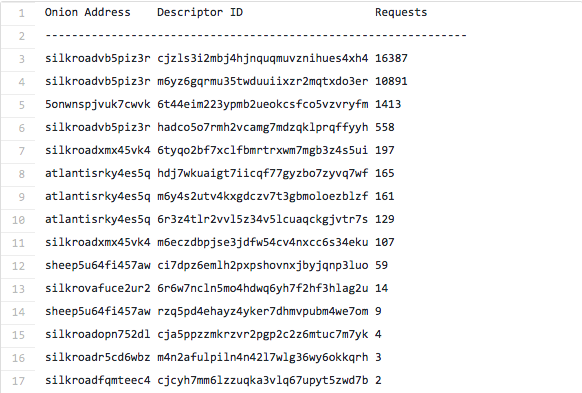
\includegraphics{images/HSDir.png}{[}8{]}

\begin{verbatim}
Un HSDir est un noeud Tor comme les autres mais il rempli une fonctionnalité supplémentaire : il reçoit les informations sur les services cachés pour signaler leur existence et permettre aux clients de les contacter. Le concensus permet à un noeud de devenir HSDir.
\end{verbatim}

\paragraph{b) Etablissement de la
connexion}\label{b-etablissement-de-la-connexion}

\begin{verbatim}
  La machine d'Alice a téléchargé les consensus et elle possède donc les IP des HSDir. Elle peut donc, toujours en utilisant le TOR, télécharger le descripteur du service caché et vérifier la signature. La machine d'Alice connait donc maintenant les IP d'introduction de mon service caché.
  [Voir annexe 3]


  Comme pour se connecter à un service publique, la machine d'Alice va choisir créér aléatoirement un circuit avec trois noeuds TOR. Le noeud de sortie sera le point de rendez-vous. La machine founira sous forme de cookie un secret à ce point de rendez-vous. Ce dernier permettra d'authentifier le service caché.
  [Voir annexe 4]

  Le machine d'Alice garde en attente ce cette connexion. Par ailleurs, elle crée un nouveau circuit de façon à ce que le noeud de sortie communique avec un point d'introduction du service caché. Elle peut ensuite communiquer à ce service : l'IP du point de rendez-vous, le secret qui a été dit à ce point de rendez-vous et la première partie de l'échange de Diffie-Hellman pour la création d'une clé symétrique entre la machine d'Alice et le service caché. Toutes ces informations sont chiffrées avec la clé publique du service caché.
  [Voir annexe 5]

  Le service caché contacte ensuite le point de rendez-vous pour s'authentifier puis en passant par ce noeud communique avec le client pour terminer l'échange de la clé symétrique de Diffie-Hellman. Maintenant, Alice et le service caché peuvent communiquer de façon sécurisé. Il n'y a pas trois noeuds Tor sur leur circuit mais 6. Les trois premiers enlèves chacun une couche de chiffrement et les trois derniers en remettent chacun une. La connexion est chiffrée du client au service caché.
  [Voir annexe 6]
\end{verbatim}

\subsubsection{6) Les Vulnérabilités de
Tor}\label{les-vulnuxe9rabilituxe9s-de-tor}

\paragraph{a) Vulnérabilité exploitant le
JavaScript}\label{a-vulnuxe9rabilituxe9-exploitant-le-javascript}

Le JavaScript est un langage de programmation utilisé par la majorité
des site web. Ce langage est exécuté côté client. Il est dangereux car
il existe des exploits javascript qui peuvent être envoyés par le
serveur pour faire exécuter du code malicieux par votre ordinateur. Par
exemple, il est possible d'injecter du code javascript exploitant la
vulnérabilité par l'hébergeur de service cachés. Ensuite, le code
éxécuté par la machine cible de l'utilisateur (le payload) récupère le
nom de la machine et l'adresse mac, et l'envoie sur un serveur via une
connexion non torrifiée, ce qui permet également de récupérer l'IP
réelle. Il est donc vivement conseiller de désactiver le JavaScript si
l'on veut utiliser le TOR en toute sécurité. Cela peut être un gros
inconvénient pour consulter des sites publiques car la plupart ne
fonctionne pas sans JavaScript, cependant les services cachés, pour la
plupart, n'utilise pas ce langage. réf : {[}1{]}

\paragraph{b) Ecoute du noeud de
sortie.}\label{b-ecoute-du-noeud-de-sortie.}

Si l'on contrôle un noeud de sortie ou que l'on est l'homme du milieu
entre un site web publique et un noeud de sortie TOR, nous avons accès
au traffic en clair. Dans les requêtes, il peut se trouver des
informations sensibles tel que des identifiants, mots de passe ou
informations personnelles qui permettraient de vous lier à cette
requête. Cela ne fonctionne pas pour les services cachés car les données
sont chiffrés de bout en bout. Exitmap et HoneyConnector sont deux
procédés de scan des nœuds de sorties, ils ont pour but de distinguer
les noeuds qui seraient corrompus. Exitmap permet de détecter les
manipulations du traffic en établissant une connexion Tor vers un leurre
controllé par le Torproject. On sait ce qu'on envoie dans le réseau, et
on regarde ce qui arrive sur le leurre. Si le traffic a été modifié,
alors ça veut dire que le noeud de sortie modifie les trames réseau.
Honeyconnector permet de détecter le sniffage passif du traffic (C'est à
dire la récupération des information sans les modifier). Concrètement,
on envoie via Tor un couple unique ``identifiant/mot de passe'' sur un
leurre controllé par le Torproject. Ensuite, si une tentative de
connexion a lieu ulterieurement sur ce leurre, alors on sait que le
noeud de sortie par lequel ce couple d'identifiant est passé l'a
intercepté. réf : {[}1{]}

\paragraph{c) Analyse de traffic}\label{c-analyse-de-traffic}

Grâce aux multiples couches de chiffrement utilisé par TOR le message
même s'il est intercepté n'est normalement pas lisible. Cependant la
taille ou la fréquence d'envoi peuvent donner des informations sur le
type de communication ou le destinataire. Pour réaliser une analyse du
traffic il faut dans la plupart des cas avoir accès a 2/3 du traffic
soit le noeud d'entré et le noeud de sortie. Ainsi on observe un
certains motif en entrée et si l'on retrouve ce motif en sortie alors on
sait d'ou vient le message. Une attaque un peut plus complexe consiste à
faire transiter un traffic important sur un relais Tor spécifique à
destination d'un serveur détenus par l'attaquant. Quand l'attaquant
recoit le traffic il peut déduire la latence induite par son traffic sur
le relais et ainsi chercher d'autres traffics sur le réseau qui seraient
passer par ce noeud donc affecter par la même latence. Il existe des
moyens pour empecher ce genre d'attaque de fournir des résultats
cohérents et utilisables tels que rajouter du traffic parasite ou
introduire des perturbations aléatoires de débit. Le problème de ces
solutions sont leur impact sur la rapidité des connexions Tor qui sont
déjà reconnues commme relativement lentes par les utilisateurs. Tor a
pris le parti de considérer que la complexité de l'analyse et de
l'exploitation des résultats garantisait un niveau de sécurité assez
important. réf : {[}1{]}

\paragraph{c) Fingerprint de la
souris}\label{c-fingerprint-de-la-souris}

Lorsque l'on navigue sur le web cela peut paraitre banal mais la facon
de déplacer sa souris ou la manière de cliquer est différentes selon les
équipements mais aussi selon les personnes. L'analyse de ces différentes
caractéristiques pourrait permettre d'identifier de manière unique un
individu. Pour cela il faudrait disposer d'une base de données,
regroupant les caractéristiques collectées sur le web classique (de
manière non anonyme), et l'utiliser sur Tor pour désanonymiser
l'utilisateur. Ce type de vulnérabilité n'est que théorique mais il met
en évidence une éventuelle faille. De plus les processus utilisés pour
tracker ces informations nécessitent Javascript, raison de plus pour
désactiver JavaScript lorsque l'on se trouve sur Tor. réf : {[}1{]}

\paragraph{c) Faiblesse des clés
d'authentification}\label{c-faiblesse-des-cluxe9s-dauthentification}

De très nombreux relais Tor utilisent des versions de Tor anciennes qui
ne sont pas mise à jour et qui utilisent donc des clés de 1024 bits qui
sont actuellement obsolètes. Si un attaquant arrive à casser la clé du
relais Tor alors il pourrait usurper l'identité de ce dernier et forcer
les connexions à passer par lui. Certaines clés publiques permettraient
même de remonter par des procédés mathématiques à la clé privée ce qui
ne devrait jamais être possible. Les recherches menées sur les clés
permettant l'authentification montre qu'un nombre non négligeable de
relais ont vu leurs clés volontairement modifiés afin de nuire à
l'anonymat de certains services cachés. réf : {[}1{]}

Annexe 1 : 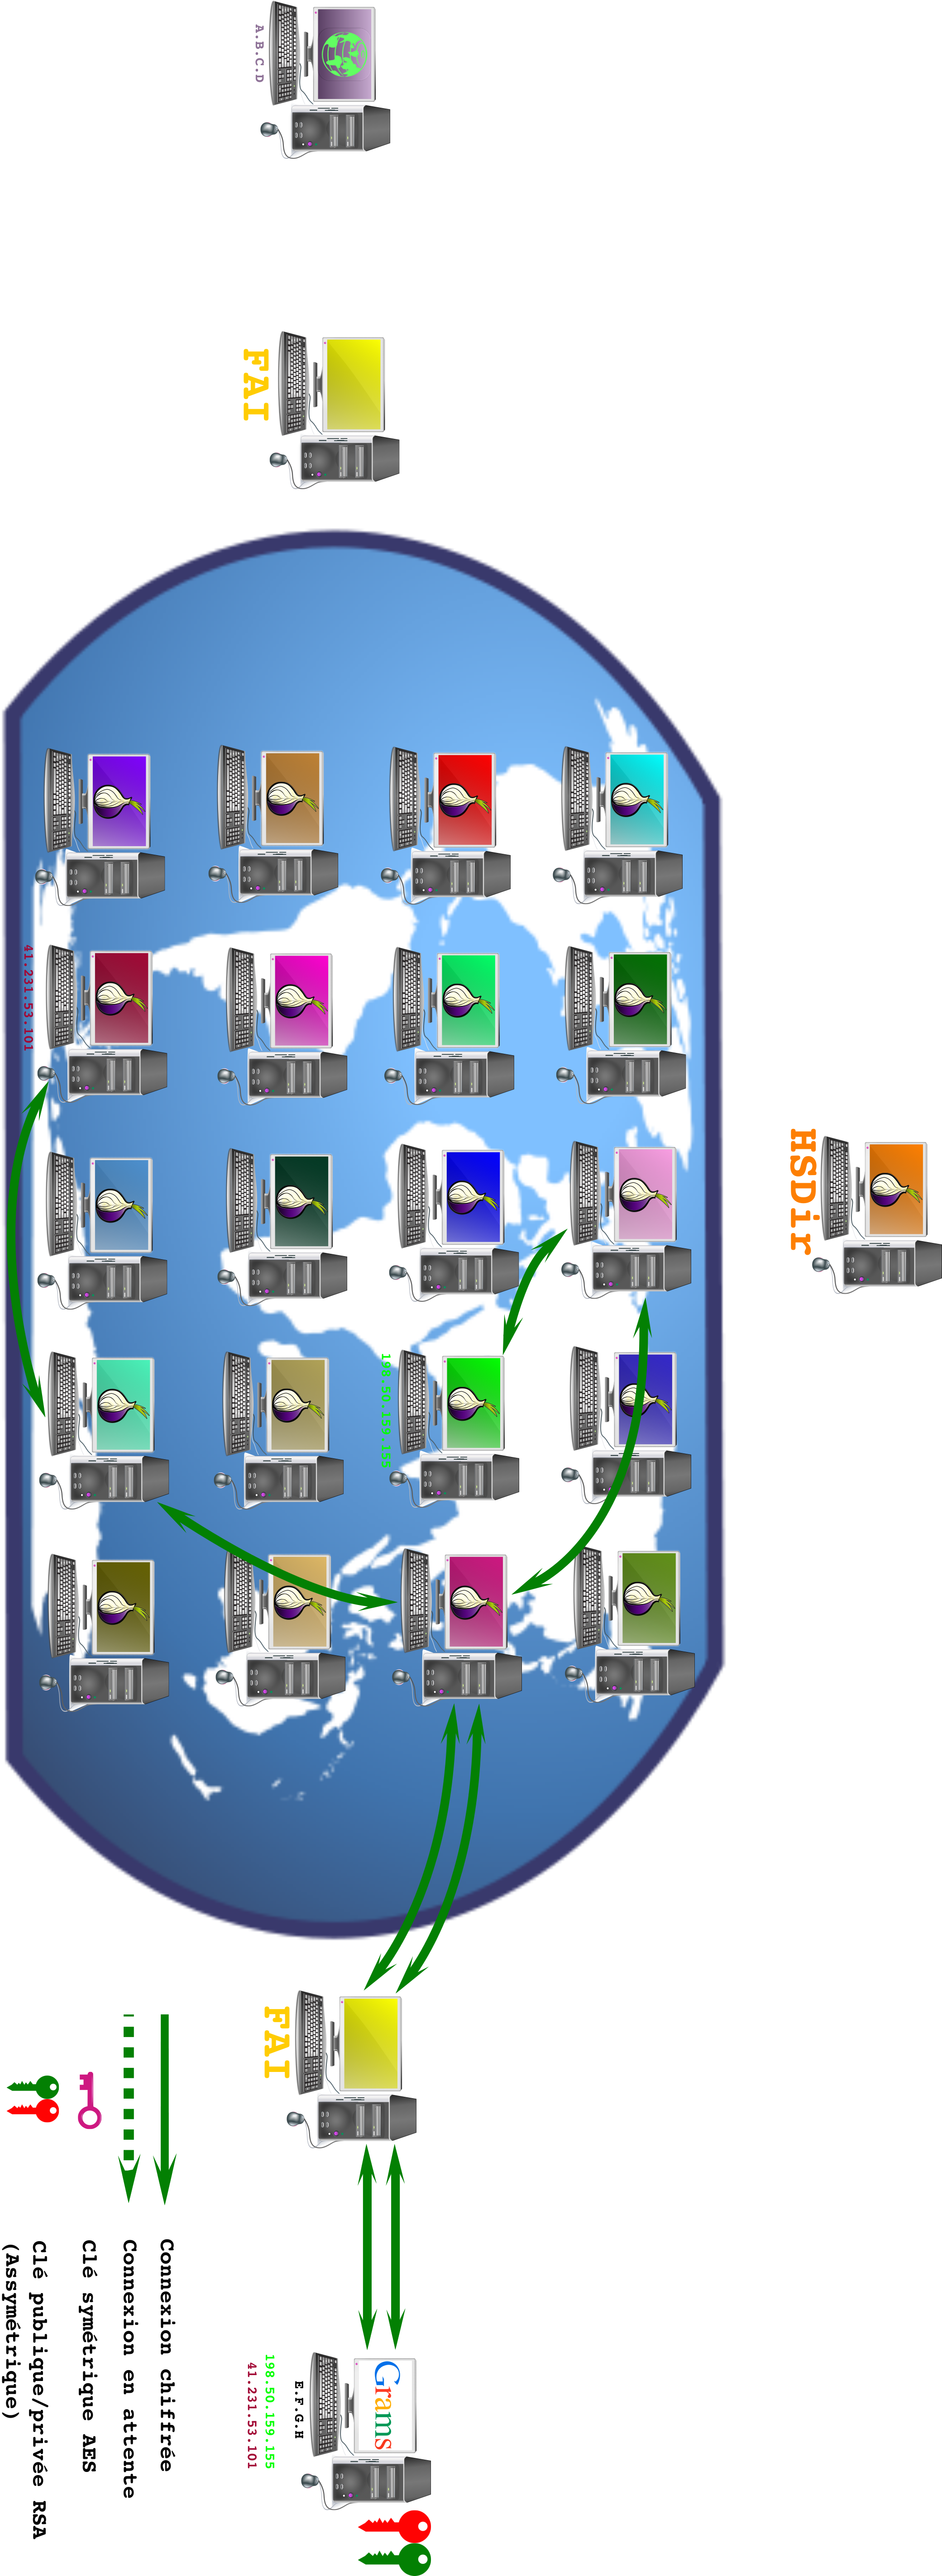
\includegraphics{images/Etablissement_circuit.png} Annexe 2 :
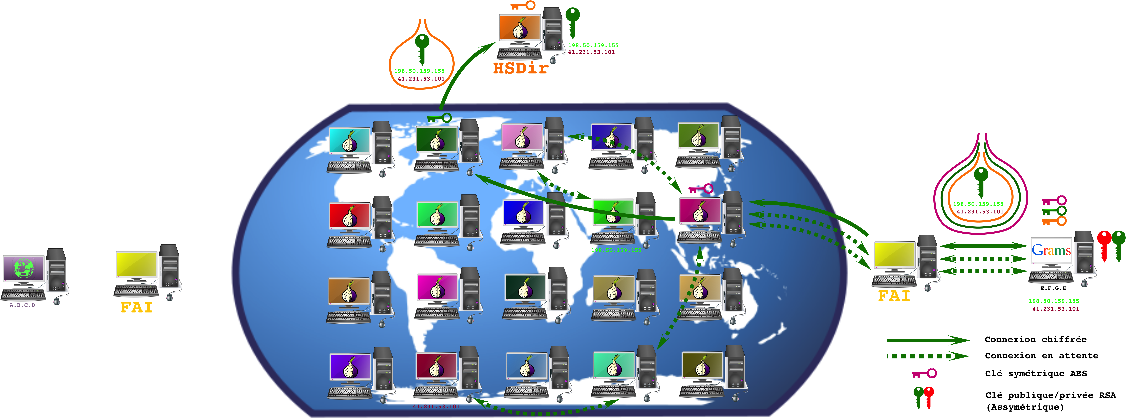
\includegraphics{images/Signalement_HSDir.png} Annexe 3 :
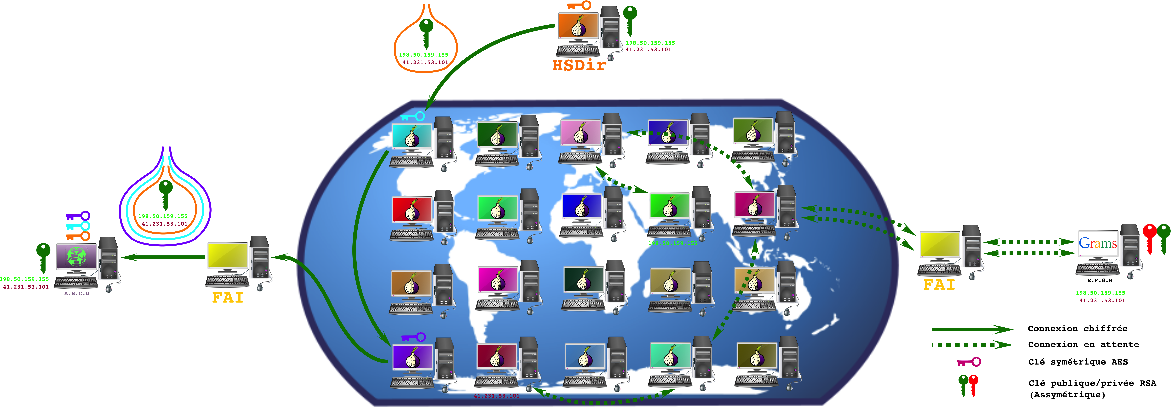
\includegraphics{images/Telechargement_Descripteur.png} Annexe 4 :
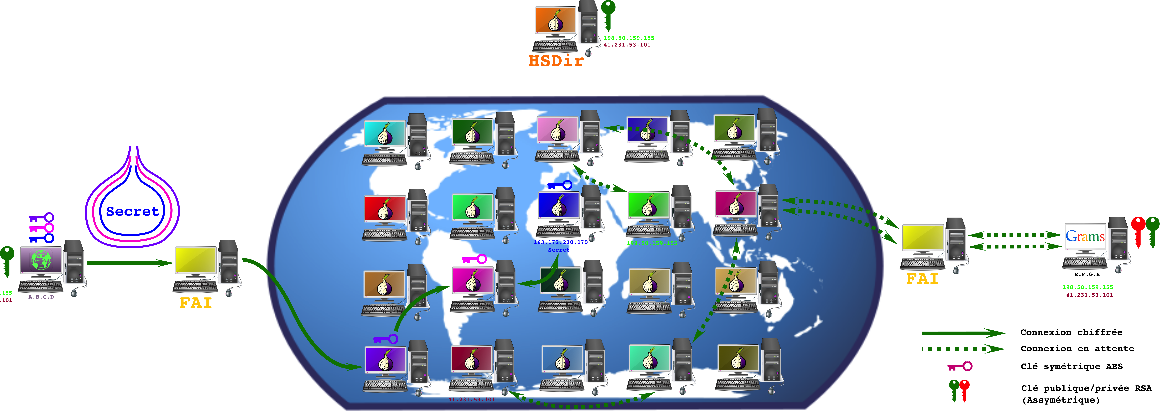
\includegraphics{images/Connexion_RDV.png} Annexe 5 :
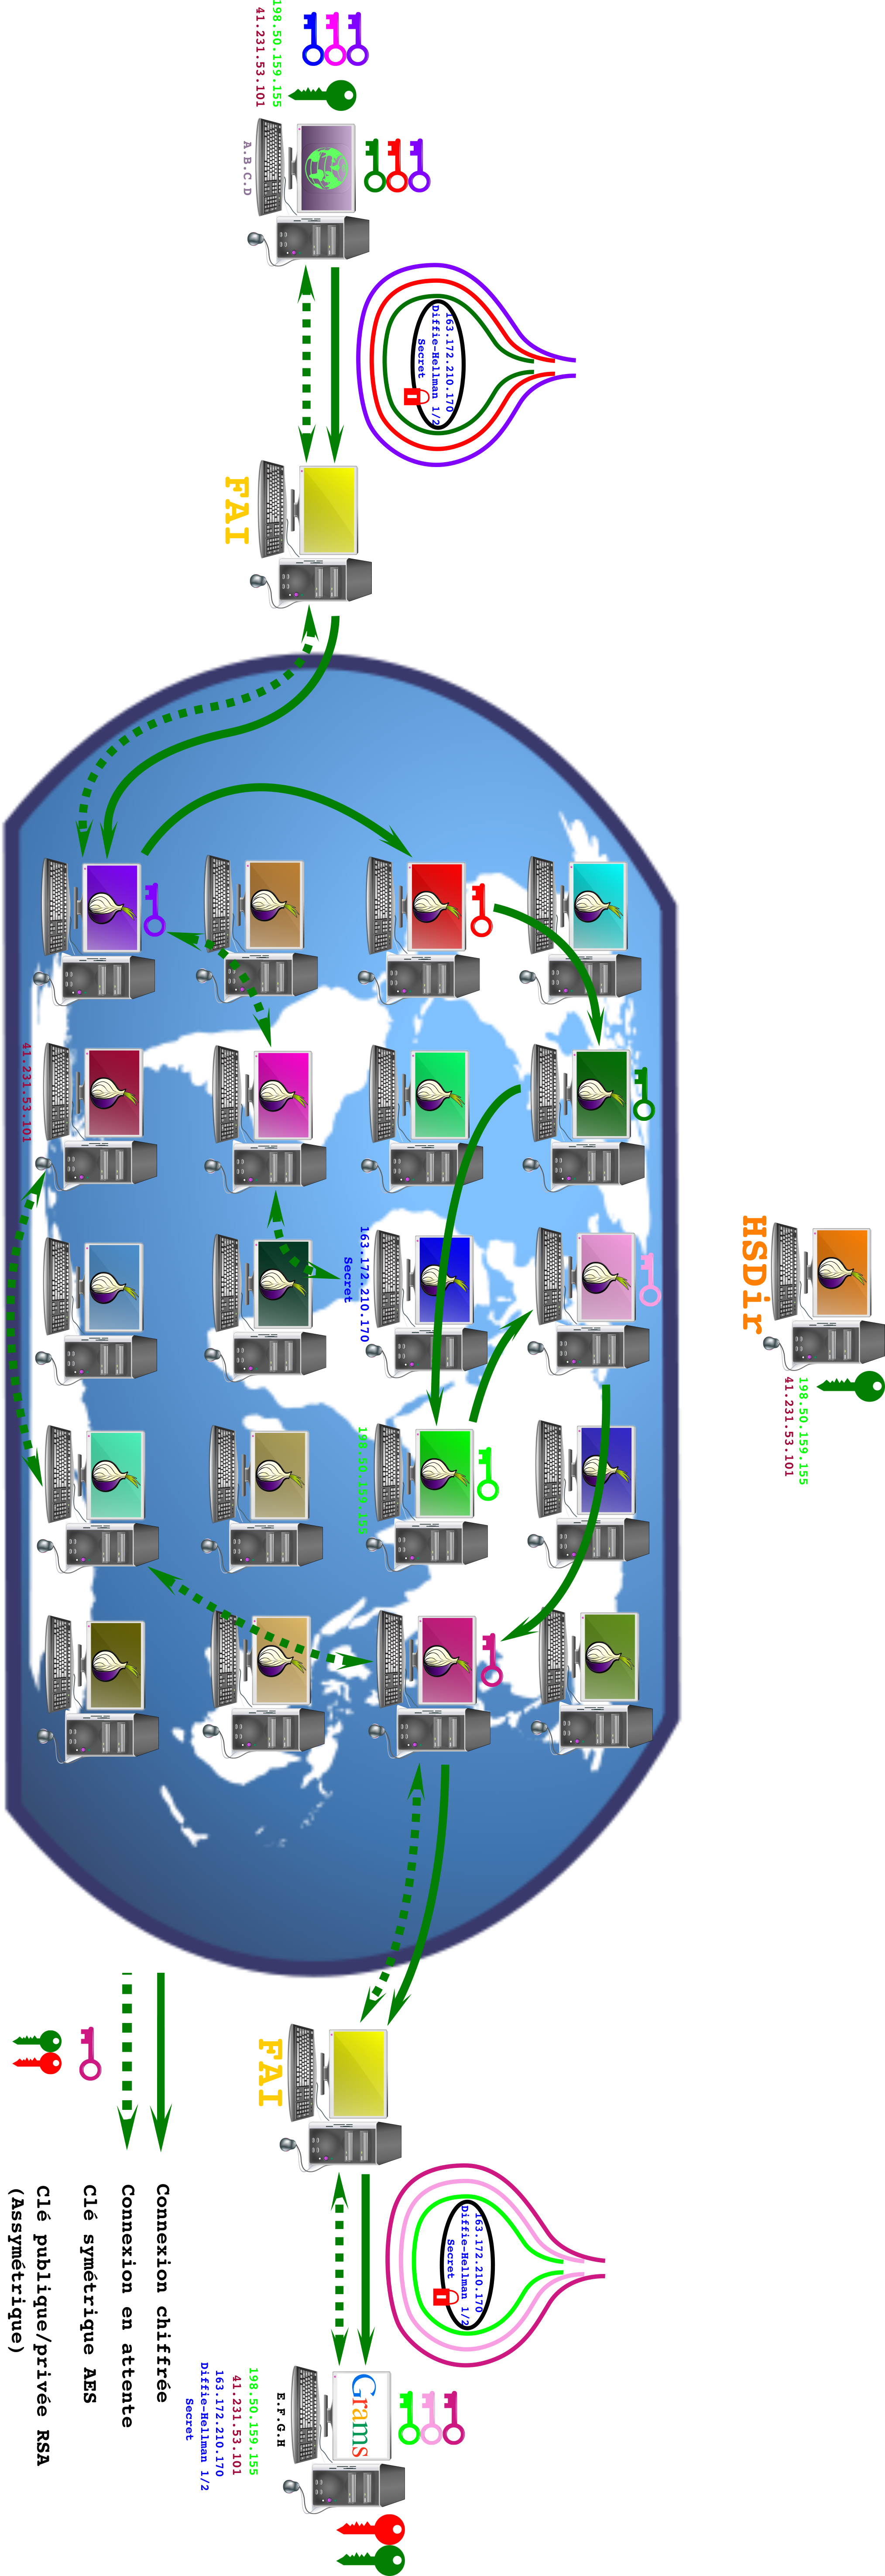
\includegraphics{images/Com_du_RDV_au_HS.png} Annexe 6 :
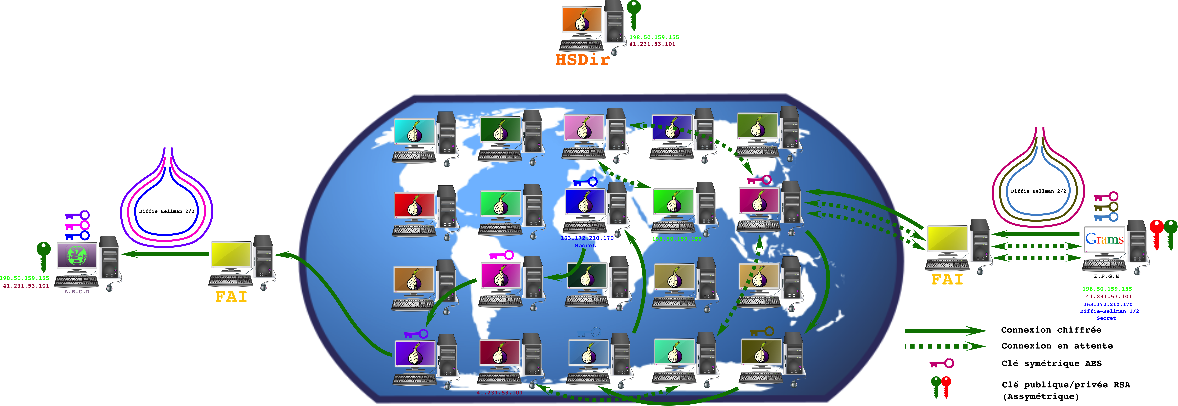
\includegraphics{images/Echange_cle_HS.png}

reference : {[}1{]} :
https://www.psychoactif.org/psychowiki/index.php?title=Tor,\_conception,\_fonctionnement\_et\_limites
{[}2{]} : https://fr.softonic.com/articles/tor-outil-navigation-anonyme
{[}3{]} : https://www.torproject.org/docs/onion-services {[}4{]} :
https://www.torproject.org/docs/tor-doc-relay.html.en\#setup {[}5{]} :
https://themimitoof.fr/mettre-en-place-un-relais-tor/ {[}6{]} :
http://www.supinfo.com/articles/single/277-creer-hidden-service-reseau-tor
{[}7{]} :http://www.ieee-security.org/TC/SP2013/papers/4977a080.pdf
{[}8{]} :https://donncha.is/2013/05/trawling-tor-hidden-services/
{[}9{]} :https://framablog.org/2016/05/06/anonymat-en-ligne-nos-oignons/
{[}10{]} : https://blog.torproject.org/lifecycle-new-relay

\end{document}
